%
% Documento: Disposições
%

\chapter{DESENVOLVIMENTO PROPOSTO}\label{chap:proj}
    O \textit{framework} proposto é baseado no conceito de PageObject, onde todas as páginas web são tratadas como objetos.
    Ainda, cada componente que seja necessário para automação, um \emph{input}, \emph{span}, etc, é um atributo desse objeto.

    Para melhor exemplificar o uso do conceito de \emph{PageObject} será utilizado como exemplo um simples login para 2
    usuários, onde será utilizada uma página que possui dois campos de texto, campo de usuário e outro de senha,
    e um botão para submeter o login.

    Primeiro, utilizou-se um exemplo básico de como o \textit{Selenium} propõe o desenvolvimento desse \emph{script} de login.
    Primeiro é iniciado o \emph{driver} do navegador, navegar para a URL, depois
    são seguidos 3 passos para cada um dos campos de texto, procurar por ele, limpar o seu conteúdo
    (porque não se sabe se ele possui algum texto pré cadastrado) e enviar os caracteres necessário para
    cada campo e por final, procurar e clicar no botão para submeter a ação do formulário. Não é um método muito viável,
    pois caso tenhamos 2 logins esse \emph{script} deverá ser duplicado para atender ambas necessidades.

    A \autoref{fig:selenium_default} exemplifica esse cenário mostrado, onde temos 2 usuários querendo a mesma coisa porém
    cada um com sua implementação.


    \begin{figure}[H]
        \vspace*{0,3cm}
        \centering
        \caption{Uso padrão Selenium}
        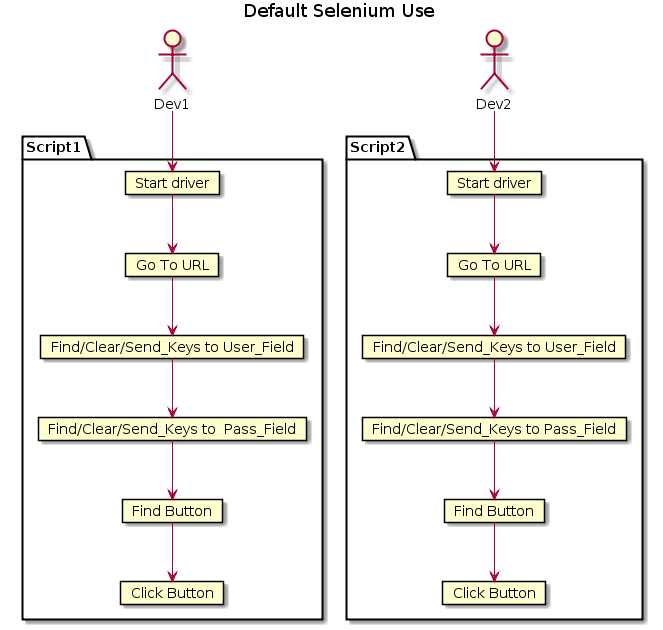
\includegraphics[width=0.9\textwidth]{./04-figuras/page_object_selenium}
        \label{fig:selenium_default}
    \end{figure}
    \vspace*{-0,9cm}
    {\raggedright \fonte{Autor desta monografia, 2017.}}

    Num segundo exemplo poderíamos separar o \emph{script} de login e criar um módulo separado para ele. Desse jeito
    os \emph{scripts} podem fazer uso do mesmo código e caso uma terceira pessoa precise dele não seria um problema.
    Porém temos todo o mapeamento dessa página preso num módulo e caso seja necessário a criação de outro
    módulo que use essa mesma pagina ainda assim teremos que duplicar mais código.

    A \autoref{fig:selenium_module} exemplifica esse cenário mostrado, onde agora temos um \emph{script} de Login
    separado dos \emph{scripts} de cada usuário.

    \begin{figure}[H]
        \vspace*{0,3cm}
        \centering
        \caption{Uso padrão Selenium com módulo}
        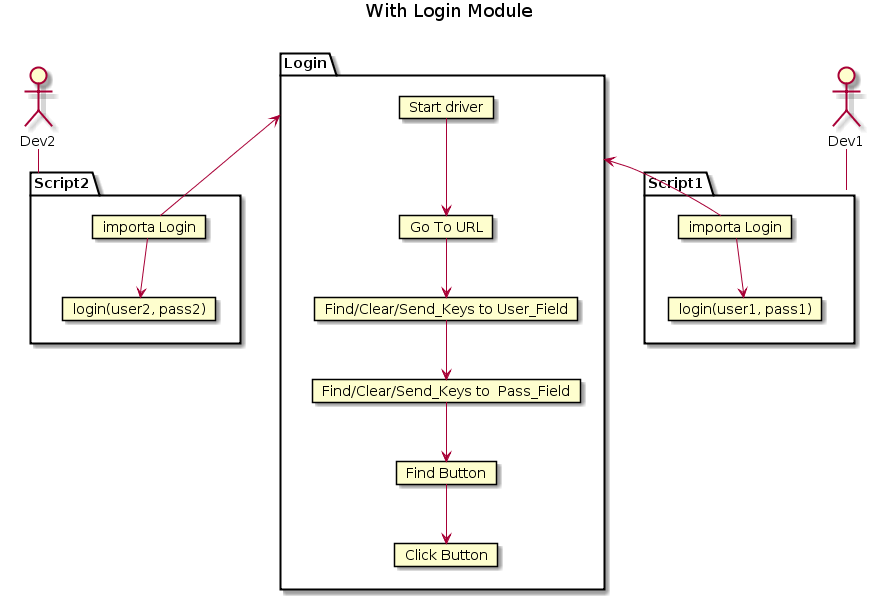
\includegraphics[width=1\textwidth]{./04-figuras/page_object_module}
        \label{fig:selenium_module}
    \end{figure}
    \vspace*{-0,9cm}
    {\raggedright \fonte{Autor desta monografia, 2017.}}

    Chegando num terceiro exemplo onde agora fazemos uso do \textit{framework} \emph{Pybot}, onde utilizando-se do
    módulo \emph{Component} (\autoref{sec:comp}) podemos separar todos os componentes da tela em atributos da nossa página
    e criar um método onde precisando de dois parâmetros ele faz o processo de login, e ainda assim, caso
    necessário pode-se utilizar os campos mapeados para fazer algum outro método sem impactar o login.
    E caso alguma referencia dos campos mapeados mude, será necessário alterar apenas um local e nenhum \emph{script}
    será impactado.

    A \autoref{fig:pybot_module} exemplifica esse cenário mostrado, onde com o uso do \emph{Pybot} a pagina de login
    é tratada como um objeto e dentro dela temos o método login para ser usado nos \emph{scripts} de cada usuário.

    \begin{figure}[H]
        \vspace*{0,3cm}
        \centering
        \caption{Uso padrão Pybot}
        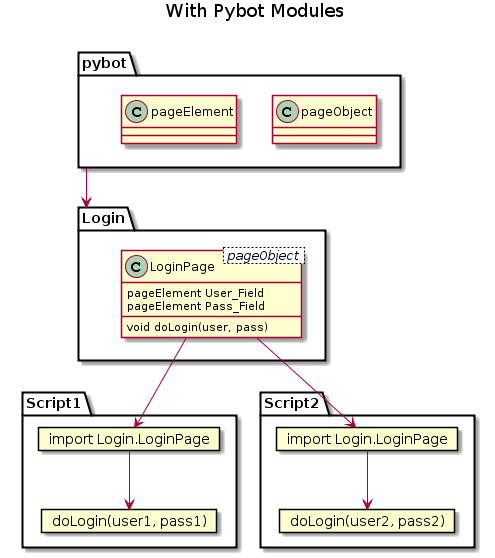
\includegraphics[width=0.8\textwidth]{./04-figuras/page_object_pybot}
        \label{fig:pybot_module}
    \end{figure}
    \vspace*{-0,9cm}
    {\raggedright \fonte{Autor desta monografia, 2017.}}